\documentclass{article}
\usepackage{amsmath,amssymb,amsthm}
\usepackage{enumerate,mathtools}
\usepackage{tikz}
\usepackage[letterpaper,margin=1in]{geometry}

% Theorems
\usepackage{amsthm}
\renewcommand\qedsymbol{$\blacksquare$}
\makeatletter
\@ifclassloaded{article}{
    \newtheorem{definition}{Definition}[section]
    \newtheorem{example}{Example}[section]
    \newtheorem{theorem}{Theorem}[section]
    \newtheorem{corollary}{Corollary}[theorem]
    \newtheorem{lemma}{Lemma}[theorem]
}{
}
\makeatother

% Random Stuff
\setlength\unitlength{1mm}

\newcommand{\insertfig}[3]{
\begin{figure}[htbp]\begin{center}\begin{picture}(120,90)
\put(0,-5){\includegraphics[width=12cm,height=9cm,clip=]{#1.eps}}\end{picture}\end{center}
\caption{#2}\label{#3}\end{figure}}

\newcommand{\insertxfig}[4]{
\begin{figure}[htbp]
\begin{center}
\leavevmode \centerline{\resizebox{#4\textwidth}{!}{\input
#1.pstex_t}}
\caption{#2} \label{#3}
\end{center}
\end{figure}}

\long\def\comment#1{}

\newcommand\norm[1]{\left\lVert#1\right\rVert}
\DeclareMathOperator*{\argmin}{arg\,min}
\DeclareMathOperator*{\argmax}{arg\,max}

% bb font symbols
\newfont{\bbb}{msbm10 scaled 700}
\newcommand{\CCC}{\mbox{\bbb C}}

\newfont{\bbf}{msbm10 scaled 1100}
\newcommand{\CC}{\mbox{\bbf C}}
\newcommand{\PP}{\mbox{\bbf P}}
\newcommand{\RR}{\mbox{\bbf R}}
\newcommand{\QQ}{\mbox{\bbf Q}}
\newcommand{\ZZ}{\mbox{\bbf Z}}
\renewcommand{\SS}{\mbox{\bbf S}}
\newcommand{\FF}{\mbox{\bbf F}}
\newcommand{\GG}{\mbox{\bbf G}}
\newcommand{\EE}{\mbox{\bbf E}}
\newcommand{\NN}{\mbox{\bbf N}}
\newcommand{\KK}{\mbox{\bbf K}}
\newcommand{\KL}{\mbox{\bbf KL}}

% Vectors
\renewcommand{\aa}{{\bf a}}
\newcommand{\bb}{{\bf b}}
\newcommand{\cc}{{\bf c}}
\newcommand{\dd}{{\bf d}}
\newcommand{\ee}{{\bf e}}
\newcommand{\ff}{{\bf f}}
\renewcommand{\gg}{{\bf g}}
\newcommand{\hh}{{\bf h}}
\newcommand{\ii}{{\bf i}}
\newcommand{\jj}{{\bf j}}
\newcommand{\kk}{{\bf k}}
\renewcommand{\ll}{{\bf l}}
\newcommand{\mm}{{\bf m}}
\newcommand{\nn}{{\bf n}}
\newcommand{\oo}{{\bf o}}
\newcommand{\pp}{{\bf p}}
\newcommand{\qq}{{\bf q}}
\newcommand{\rr}{{\bf r}}
\renewcommand{\ss}{{\bf s}}
\renewcommand{\tt}{{\bf t}}
\newcommand{\uu}{{\bf u}}
\newcommand{\ww}{{\bf w}}
\newcommand{\vv}{{\bf v}}
\newcommand{\xx}{{\bf x}}
\newcommand{\yy}{{\bf y}}
\newcommand{\zz}{{\bf z}}
\newcommand{\0}{{\bf 0}}
\newcommand{\1}{{\bf 1}}

% Matrices
\newcommand{\Ab}{{\bf A}}
\newcommand{\Bb}{{\bf B}}
\newcommand{\Cb}{{\bf C}}
\newcommand{\Db}{{\bf D}}
\newcommand{\Eb}{{\bf E}}
\newcommand{\Fb}{{\bf F}}
\newcommand{\Gb}{{\bf G}}
\newcommand{\Hb}{{\bf H}}
\newcommand{\Ib}{{\bf I}}
\newcommand{\Jb}{{\bf J}}
\newcommand{\Kb}{{\bf K}}
\newcommand{\Lb}{{\bf L}}
\newcommand{\Mb}{{\bf M}}
\newcommand{\Nb}{{\bf N}}
\newcommand{\Ob}{{\bf O}}
\newcommand{\Pb}{{\bf P}}
\newcommand{\Qb}{{\bf Q}}
\newcommand{\Rb}{{\bf R}}
\newcommand{\Sb}{{\bf S}}
\newcommand{\Tb}{{\bf T}}
\newcommand{\Ub}{{\bf U}}
\newcommand{\Wb}{{\bf W}}
\newcommand{\Vb}{{\bf V}}
\newcommand{\Xb}{{\bf X}}
\newcommand{\Yb}{{\bf Y}}
\newcommand{\Zb}{{\bf Z}}

% Calligraphic
\newcommand{\Ac}{{\cal A}}
\newcommand{\Bc}{{\cal B}}
\newcommand{\Cc}{{\cal C}}
\newcommand{\Dc}{{\cal D}}
\newcommand{\Ec}{{\cal E}}
\newcommand{\Fc}{{\cal F}}
\newcommand{\Gc}{{\cal G}}
\newcommand{\Hc}{{\cal H}}
\newcommand{\Ic}{{\cal I}}
\newcommand{\Jc}{{\cal J}}
\newcommand{\Kc}{{\cal K}}
\newcommand{\Lc}{{\cal L}}
\newcommand{\Mc}{{\cal M}}
\newcommand{\Nc}{{\cal N}}
\newcommand{\Oc}{{\cal O}}
\newcommand{\Pc}{{\cal P}}
\newcommand{\Qc}{{\cal Q}}
\newcommand{\Rc}{{\cal R}}
\newcommand{\Sc}{{\cal S}}
\newcommand{\Tc}{{\cal T}}
\newcommand{\Uc}{{\cal U}}
\newcommand{\Wc}{{\cal W}}
\newcommand{\Vc}{{\cal V}}
\newcommand{\Xc}{{\cal X}}
\newcommand{\Yc}{{\cal Y}}
\newcommand{\Zc}{{\cal Z}}

% Bold greek letters
\newcommand{\alphab}{\hbox{\boldmath$\alpha$}}
\newcommand{\betab}{\hbox{\boldmath$\beta$}}
\newcommand{\gammab}{\hbox{\boldmath$\gamma$}}
\newcommand{\deltab}{\hbox{\boldmath$\delta$}}
\newcommand{\etab}{\hbox{\boldmath$\eta$}}
\newcommand{\lambdab}{\hbox{\boldmath$\lambda$}}
\newcommand{\epsilonb}{\hbox{\boldmath$\epsilon$}}
\newcommand{\nub}{\hbox{\boldmath$\nu$}}
\newcommand{\mub}{\hbox{\boldmath$\mu$}}
\newcommand{\zetab}{\hbox{\boldmath$\zeta$}}
\newcommand{\phib}{\hbox{\boldmath$\phi$}}
\newcommand{\psib}{\hbox{\boldmath$\psi$}}
\newcommand{\thetab}{\hbox{\boldmath$\theta$}}
\newcommand{\taub}{\hbox{\boldmath$\tau$}}
\newcommand{\omegab}{\hbox{\boldmath$\omega$}}
\newcommand{\xib}{\hbox{\boldmath$\xi$}}
\newcommand{\sigmab}{\hbox{\boldmath$\sigma$}}
\newcommand{\pib}{\hbox{\boldmath$\pi$}}
\newcommand{\rhob}{\hbox{\boldmath$\rho$}}

\newcommand{\Gammab}{\hbox{\boldmath$\Gamma$}}
\newcommand{\Lambdab}{\hbox{\boldmath$\Lambda$}}
\newcommand{\Deltab}{\hbox{\boldmath$\Delta$}}
\newcommand{\Sigmab}{\hbox{\boldmath$\Sigma$}}
\newcommand{\Phib}{\hbox{\boldmath$\Phi$}}
\newcommand{\Pib}{\hbox{\boldmath$\Pi$}}
\newcommand{\Psib}{\hbox{\boldmath$\Psi$}}
\newcommand{\Thetab}{\hbox{\boldmath$\Theta$}}
\newcommand{\Omegab}{\hbox{\boldmath$\Omega$}}
\newcommand{\Xib}{\hbox{\boldmath$\Xi$}}

% mixed symbols
\newcommand{\sinc}{{\hbox{sinc}}}
\newcommand{\diag}{{\hbox{diag}}}
\renewcommand{\det}{{\hbox{det}}}
\newcommand{\trace}{{\hbox{tr}}}
\newcommand{\tr}{\trace}
\newcommand{\sign}{{\hbox{sign}}}
\renewcommand{\arg}{{\hbox{arg}}}
\newcommand{\var}{{\hbox{var}}}
\newcommand{\cov}{{\hbox{cov}}}
\renewcommand{\Re}{{\rm Re}}
\renewcommand{\Im}{{\rm Im}}
\newcommand{\eqdef}{\stackrel{\Delta}{=}}
\newcommand{\defines}{{\,\,\stackrel{\scriptscriptstyle \bigtriangleup}{=}\,\,}}
\newcommand{\<}{\left\langle}
\renewcommand{\>}{\right\rangle}
\newcommand{\Psf}{{\sf P}}
\newcommand{\T}{\top}
\newcommand{\m}[1]{\begin{bmatrix} #1 \end{bmatrix}}


\setlength{\parindent}{0pt}

\begin{document}

\begin{center}
  \Large\textbf{Convex Optimization Overview}\\
  \large\textit{Conner DiPaolo}
\end{center}
\vspace*{1em}

\tableofcontents
\vspace{1em}

\section{Introduction}

Convex optimization in a large way influences the way
people think about and phrase machine learning problems.
Almost all problems we will see in our studies are developed
or can be viewed as optimization problems. Some problems,
like the Support Vector Machine you will all see in the coming
weeks, are almost entirely based in the heart of convex optimization.\\

We don't plan on bringing you all up to speed completely on
the art of Convex Optimization, but hopefully in two sections you
will know enough to be able to think about problems in new, interesting
ways that will aid your studies in and out of machine learning.\\

The only real prerequisite for this material is a strong confidence
in linear algebra and familiarity with matrix calculus.

%%%%%%%%%%%%%%%%%%%%%%%%%%%%%%%%%%%%%%%%%%%%
\section{Convex Sets}



The first step into examining convexity is defining what a
\textbf{convex set} is when given, for example, a subset of the real numbers,
or the set of matrices.

\begin{figure}
    \centering
    \begin{center}
        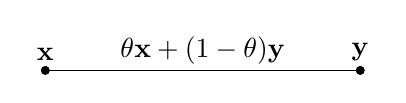
\begin{tikzpicture}
            \draw[fill=black] (0,0) circle (0.05) node[above] {$\xx$};
            \draw[fill=black] (4,0) circle (0.05) node[above] {$\yy$};
            \draw (0,0) -- (4,0);
            \draw (2,0.25) node {$\theta\xx + (1-\theta)\yy$};
        \end{tikzpicture}
    \end{center}
    \caption{\textbf{Convex Combination}. The line segment between $\xx$ and $\yy$ 
    above represents every possible combination $\{\theta\xx + (1-\theta)\yy : 
    0\leq\theta\leq1\}$.}
    \label{fig:convex-comb}
\end{figure}

\begin{definition}[Convex Combination]
    In the $n=2$ case, the convex combination of points $\xx$ and $\yy$ in an
    affine space is
    \[
        \theta\xx + (1-\theta)\yy
    \]
    where $0\leq\theta\leq1$. Intuitively, this is the line segment between
    $\xx$ and $\yy$ (consider $\theta=0$ and $\theta=1$), as seen in Figure
    \ref{fig:convex-comb}. More generally,
    a convex combination of points $\xx_1,\xx_2,\dots,\xx_n$ in an affine space (vector
    spaces included) is the combination
    \[
        \thetab_1\xx_1 + \thetab_2\xx_2 + \dots + \thetab_n\xx_n = \thetab^\T\xx
    \]
    where $\theta_i \geq 0$ and $\1^\T\theta = 1$. That is, $\thetab$ lies on the
    standard probability simplex.  
\end{definition}

With this definition of a convex combination we can define
a convex set:

\begin{figure}
    \centering
    \begin{center}
        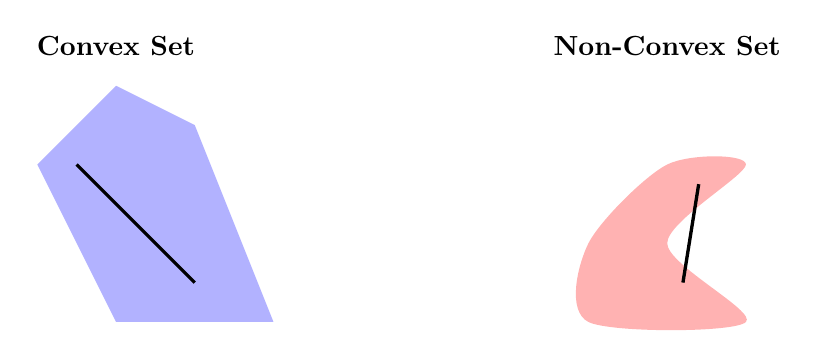
\begin{tikzpicture}
            \begin{scope}[shift={(-3,0)}]
                \draw (0,3.5) node {\textbf{Convex Set}};
                \fill[color=blue!30] (0,0) -- (-1,2) -- (0,3) -- (1,2.5) -- (2,0)  -- cycle;
                \draw[very thick] (-0.5,2) -- (1,0.5);
            \end{scope}
            \begin{scope}[shift={(3,0)}]
                \draw (1,3.5) node {\textbf{Non-Convex Set}};
                \fill[color=red!30] plot [smooth cycle] coordinates {(0,1) (1,2) (2,2) (1,1) (2,0) (0,0)};
                \draw[very thick] (1.4,1.75) -- (1.2,0.5);
            \end{scope}
        \end{tikzpicture}
    \end{center}
    \caption{{\bf Set convexity.} Intuitively, a set is convex
    if a line drawn between any two points within the set lies completely in the set. The convex set
    to the left is a \textit{convex hull} of it's vertices, meaning the set is constructed
    as all possible convex combinations of its vertices. These sets are subsets of $\RR^2$.}
    \label{fig:convex-sets}
\end{figure}

\begin{definition}[Convex Set]
    A set $C$ is convex if, given $\xx,\yy \in C$, every convex combination
    of $\xx$ and $\yy$ is still in $C$. Mathematically,
    \[
        \theta\xx + (1-\theta)\yy \in C. \tag{$0\leq\theta\leq1$}
    \]
    See Figure \ref{fig:convex-sets} for an illustration. Intuitively, this
    means that every line segment between any two points in $C$ is contained
    entirely within $C$.
\end{definition}

\subsection{Examples of Convex and Non-Convex Sets}

\begin{example}[All of $\RR^n$ is convex.]
    $\RR^n$ is convex.
\end{example}
\begin{proof}
    As a vector space, for any $\theta_1,\theta_2 \in \RR$ and $\xx$ and
    $\yy$ in $\RR^n$,
    \[
        \theta_1 \xx + \theta_2 \yy \in \RR^n.
    \]
    Thus, restricting $\theta_2 = 1-\theta_1$ and $0\leq\theta_1\leq1$
    does not change this fact, and any convex combination is also in
    $\RR^n$, making the set convex by definition.
\end{proof}

\begin{example}[The Non-Negative Orthant $\RR^n_+$]
    The set of all vectors
    \[
        \{\xx : \xx\in\RR^n \text{ and } \xx_i \geq 0\}
    \]
    is convex.
\end{example}
\begin{proof}
    Left as an exercise to the reader.
\end{proof}

\begin{example}[Closed Intervals in $\RR$ are Convex]
    Let $C = [a,b]$ be a subset of the real numbers where $a \leq b$.
    Then $C$ is convex.
\end{example}
\begin{proof}
    Suppose, without loss of generality, that $x_1 \leq x_2$ where
    $x_1,x_2 \in [a,b]$. Now let $0\leq\theta\leq1$. Then
    \[
        \theta x_1 + (1-\theta) x_2 \leq \theta x_2 + (1-\theta) x_2 = x_2
    \]
    because $\theta x_1 \leq \theta x_2$. Similarly,
    \[
        \theta x_1 + (1-\theta) x_2 \geq \theta x_1 + (1-\theta) x_1 = x_1
    \]
    because $(1-\theta) x_2 \geq (1-\theta) x_1$. Thus
    \[
        a \leq x_1 \leq \theta x_1 + (1-\theta) x_2 \leq x_2 \leq b,
    \]
    and hence
    \[
        \theta x_1 + (1-\theta) x_2 \in [a,b].
    \]
    Therefore, by the definition of convexity, $[a,b]\subseteq\RR$ is convex
    for any $a \leq b$.
\end{proof}

\begin{example}[The Set of All Complex Hermetian Matrices is Convex]
    \label{ex:hermitian-convex}
    Let $C = \{A : A\in\CC^{n\times n} \text{ and } A^* = A\}$. $C$ is
    convex.
\end{example}
\begin{proof}
    Let $A,B\in\CC^{n\times n}$ be Hermitian matrices and $0\leq\theta\leq1$.
    Then
    \begin{align}
        (\theta A + (1-\theta) B)^* &= (\theta A)^* + \left[(1-\theta)B\right]^*\\
        &= \theta A^* + (1-\theta) B^*\\
        &= \theta A + (1-\theta) B \tag{because $A^*=A$ and $B^*=B$}\\
    \end{align}
    Thus every convex combination of Hermitian matrices is Hermitian,
    and by the definition of convexity the set is convex.
\end{proof}

\begin{corollary}[The Set of All Real Symmetric Matrices is Convex]
    Let $C = \{A : A\in\RR^{n\times n} \text{ and } A^\T = A\}$. $C$ is
    convex.
\end{corollary}
\begin{proof}
    Left as an exercise to the reader.
\end{proof}

\begin{example}[The Set of All Linear Matrix Inequalities is Convex]
    Let $A_i$ and $B$ be symmetric $n\times n$ matrices and
    $\xx\in\RR^n$.
    Let $C = \{\xx : A(\xx) \preceq B\}$ where $A(\xx) = \xx_1A_1 +
    \dots + \xx_kA_k$. $C$ is convex.
\end{example}
\begin{proof}
    Let $0\leq\theta\leq1$ and $\xx, \yy \in C$. Then
    \begin{align*}
        A(\theta\xx + (1-\theta)\yy) &= \sum_i \left[ \theta\xx_i + (1-\theta)\yy_i \right]A_i\\
        &= \theta\sum_i \xx_i A_i + (1-\theta)\sum_i \xx_i A_i\\
        &= \theta A(\xx) + (1-\theta) A(\yy)\\
        &\leq \theta B + (1-\theta) B\\
        &= B.
    \end{align*}
    Thus any convex combination of elements of $C$ is contained
    in $C$ and by definition $C$ is convex.
\end{proof}

\begin{example}[The Space of Probability Distributions is Convex]
    Let $\Pc$ be the space of continuous probability distributions over
    $\RR^n$. That is, every element of $\Pc$ defines a unique probability
    density function $\PP(x) \geq 0$ such that \[\int_{\RR^n} \PP(x) dx=1.\]
    $\Pc$ is convex.
\end{example}
\begin{proof}
    Let $f$ and $h$ be valid probability distributions from $\Pc$. That is,
    \[
        f,h \in \left\{\PP(x) : \int_{\RR^n} \PP(x)dx = 1 \text{ and } \PP(x) \geq 0 \right\}.
    \]
    Now let $0\leq\theta\leq1$. Then
    \[
        \theta f(x) + (1-\theta) h(x) \geq 0
    \]
    as a positive combination of positive functions. Similarly,
    \begin{align*}
        \int_{\RR^n}\left[ \theta f(x) + (1-\theta) h(x) \right]dx &= \theta\int_{\RR^n}f(x)dx + (1-\theta)\int_{\RR^n}h(x)dx\\
        &= \theta + (1-\theta) = 1.
    \end{align*}
    Thus every convex combination of probability distributions over $\RR^n$ is
    a valid distribution (often called a mixture), and therefore the set of
    all valid probability distributions over $\RR^n$ is convex itself.
\end{proof}

\begin{example}[Disjoint Intervals in $\RR$ are Not Convex]
    Let $N = [a,b] \cup [c,d]$ where $a\leq b < c \leq d$.
    $N$ is \textbf{not} convex.
\end{example}
\begin{proof}
    Let $b,c\in N$ be as described above. Then for $0<\theta<1$
    (not we aren't including inequality),
    \[
        \theta b + (1-\theta)c \not\in N.
    \]
    Thus not \textit{every} convex combination of elements in
    $N$ is in $N$, and $N$ is not convex.
\end{proof}

\section{Convex Functions}

\subsection{First Order Conditions: $f(x) \geq f(y) + \nabla f(y)^\T (x-y)$}

\subsubsection{Examples On Determining Convexity}

\subsection{Second Order Conditions: $\nabla^2 f \succeq 0$}

\subsubsection{More Examples On Determining Convexity}

\subsection{Concavity and Linearity}

%%%%%%%%%%%%%%%%%%%%%%%%%%%%%%%%%%%%%%%%%%%%
\section{Optimization Problems}

\subsection{Convex Optimization Problems}

\subsubsection{Linear Programs}

\subsubsection{Quadratic Programs}

\subsubsection{Global Optimality of a Convex Optimum}

\subsection{Optimal Flow As a Convex Optimization Problem}

%%%%%%%%%%%%%%%%%%%%%%%%%%%%%%%%%%%%%%%%%%%%
\section{Algorithms for Solving Convex Problems}

\subsection{Gradient Descent}

\subsection{Newton's Method}

%%%%%%%%%%%%%%%%%%%%%%%%%%%%%%%%%%%%%%%%%%%%
\section{Duality}

\subsection{Duality Gap}

\subsection{The Lagrange Dual Function}

\subsection{Finding the Dual}

\subsubsection{The Dual of The Linear Program}

\subsection{Solving Problems Using Duality}

\subsubsection{Minimize a Quadratic Under Quadratic Constraints}

\subsection{Complementary Slackness of Duality}

\subsubsection{Solving The Dual Linear Program via a Primal Solution}

\subsection{The KKT (Karush-Kuhn-Tucker) Conditions}


\end{document}
